\cotefile{1}

\scanpage{98}

\[
\sum|x_i x_i'|\leq N(x)N'(x')\unsure{)}\tag*{(10)}
\]

En effet, on a $\sum_{1}^{n}|x_i x_i'|=\langle |x|_n,|x'|_n\rangle\leq N(|x|_n)N(|x'|_n)\leq N(x)N'(x')$\unsure{)}, d'où (10). Il en résulte un \uline{accouple-}\newline\uline{ment} entre $\ell^N$ et $\ell^{N'}$, \deleted{\unsure{qui} \inserted{\unsure{est}}} \inserted{d'où en restreignant} \uline{entre $\ell_N$ et $\ell^{N'}$}; \deleted{\unsure{cet accoupl} \unsure{on a ainsi associé à $\ell$ de $\ell^{N'}$} \unsure{i.e. une application|une forme} linéaire continue \inserted{\unsure{de norme} $\leq 1$}, $\ell^{N'}$ dans $(\ell_N)'$} \unsure{je dis} que \uline{le dual de $\ell_N$ s'identifie exactement à $\ell^{N'}$} (avec sa norme) par cet accouplement.

\margin{\textcolor{red}{!}\quad\tikz[baseline=-.6ex]{\draw[red,line width=.7pt] (0,0)--(0,.6);}}

En effet, \deleted{\unsure{soit la}} il suffit de montrer qu'une forme linéaire continue $X'$ sur $\ell_N$ est définie par un \inserted{$x'$} élément de $\ell^{N'}$ \deleted{de \illegible{1}} tel que $N'(x')\leq\lVert X'\rVert$.

En effet, $X'$ \deleted{\unsure{est entièrement} \inserted{\unsure{dé|aussi}}} il suffit de le voir pour la \deleted{\unsure{part}} restriction à $\ell^1$, alors $X'$ \inserted{est} défini \deleted{\unsure{p|par}} \inserted{par} un $x'\in\ell^\infty$, \deleted{\unsure{avec}} on a $N'(|x'|_n)\leq\lVert X'\rVert$, d'où aussitôt $N'(x')\leq\lVert X'\rVert$, et le résultat.

-- Notons qu'en général, le dual de $\ell^N$ n'est pas $\ell^{N'}$, \deleted{\unsure{car}} car $\ell_N$ ne sera pas dense dans $\ell^N$. Ex\,: $N=N_\infty$. Notons que

\margin{\uline{Prop}}
\uline{pour que $\ell_N$ soit réflexif, il faut et il suffit que $\ell^N$ resp$^t$ $\ell_{N'}$ resp$^t$ $\ell^{N'}$ le soit}. \inserted{\uline{Il faut et il suffit pour cela que l'on ait $\ell_N=\ell^N$} \uuline{et} \uline{$\ell_{N'}=\ell^{N'}$.}} \deleted{En effet,}

$\ell^N$ réflexif implique $\ell_N$ réflexif (sous-espace fermé) qui implique $\ell^{N'}$ réflexif (dual de $\ell_N$) qui \inserted{de même} implique $\ell_{N'}$ réflexif et lui-$=$ implique $\ell^N$ réflexif, ce qui achève la démonstration \deleted{de l'équivalence pour} circulaire de l'équivalence des 4 conditions. Alors $\ell_{N'}$, qui est un sous-espace \deleted{\unsure{fort}} \uline{total} \inserted{et fortement fermé} du dual $\ell^{N'}$ de $\ell_N$, est identique à $\ell^{N'}$, et pour la $=$ raison on aura $\ell_N=\ell^N$.

\margin{\textcolor{red}{?}}

\inserted{Réciproquement,} s'il en est ainsi, alors le dual de $\ell_N$ est $\ell^{N'}=\ell_{N'}$, et le dual de ce dernier est $\ell^N=\ell_N$, donc $\ell_N$ coïncide avec son bidual, et est donc réflexif.

\inserted{Soit $N$ une norme de Schatten sur $R^{(N)}$ \deleted{non équivalente à $N_\infty$}\inserted{non équivalente à $N_\infty$}.} Soient $E,F$ deux espaces de Hilbert, \deleted{\unsure{$N$|si}} on désigne par $L^{\deleted{\unsure{N}}N}_{\deleted{\unsure{0}}}(E,F)$ le \deleted{\unsure{sous|l'espace}} sous-espace de $L_0(E,F)$ formé des $u$ tels que $\unsure{(\rho_i(u))|(\rho_i u)}\in\ell^N$, i.e. tels que

\[
N(u)=N(\unsure{(\rho_i(u))|(\rho_i u)})<+\infty\tag*{(11)}
\]

\margin{99}


\scanpage{99}

\deleted{Si $N$ est \unsure{équivalente à la}} \deleted{Sous ces conditions,}

Alors la fonction $u\to N(u)$ sur $L^N_{\deleted{\unsure{0}}}(E,F)$ est une \uline{norme}. En effet, on a $N(u+v)=\lim_{n\to\infty}N(|(\rho_i(u+v))|_n)\deleted{\unsure{,\rho_2(u+v)}}$, or le second mb est majoré par $N(|(\rho_i(u))|_n)\deleted{\unsure{,\rho_2(u)}}+N(|(\rho_i(v))|_n)\deleted{\unsure{,\rho_2(v)}}$ (N\textsuperscript{o} , formule (44)), donc par $N(u)+N(v)$. On note aussi trivialement $N(\lambda u)=|\lambda|N(u)$, et $N(u)=0\Rightarrow u=0$.

\margin{$N(u)=N(u^*)$ (12)\par $\left.\begin{aligned}N(uv)&\leq\lVert u\rVert N(v)\\N(vu)&\leq\lVert u\rVert N(v)\end{aligned}\right\}$ (13)}

L'espace $L^N_{\deleted{\unsure{0}}}(E,F)$ est donc un espace normé; \deleted{\unsure{prouvons qu'il est \uline{complet}.}}\inserted{soit} $L_N(E,F)$ le sous-espace normé formé des $u$ tels que $\unsure{(\rho_i(u))|(\rho_i u)}\in\ell_N$. Je dis que $L_N(E,F)$ est l'adhérence de $\overline E\otimes F$ dans $L^N(E,F)$. En effet, montrons que

$\sum\rho_i\bar e_i\otimes f_i$ est limite au sens de $N$ de $\sum_1^n\rho_i\bar e_i\otimes f_i$, donc que $N(\sum_{n+1}^\infty\rho_i\bar e_i\otimes f_i)=N(\rho_{n+1}\unsure{(u)},\ldots)\to 0$ pour $n\to+\infty$, en d'autres termes, que dans $\ell_N$ les opérations $x\to t_n(x)=(\overbrace{0{-}0}^{n},x_{n+1},x_{n+2}\unsure{-})$ tendent vers $0$ simplement. Or elles forment une suite équicontinue, qui tend vers zéro dans \deleted{\unsure{un}} $R^{(N)}$, ce qui prouve la chose. \deleted{\unsure{Notons} \unsure{donc|$N_\infty$}, \unsure{lorsqu'on a} $L^N(E,F)$ \unsure{et si|et que} $N$ \illegible{3}}

\margin{Définition de $L^N(E,F)$ si $N\simeq N_\infty$ ($L^N(E,F)=L(E,F)$, avec \textcircled{14} $\boxed{N(u)=\underset{\substack{v\in F'\otimes E\\N^\circ(v)\leq 1}}{\operatorname{Sup}}\operatorname{Tr}(vu)}$ $L_N(E,F)$ comme avant). Cas où $u$ est cpt.}

\deleted{Le dual de $L_N(E,F)$ s'identifie à un sous-espace du dual de $L_{N_1}(E,F)=L^1(E,F)$, donc de $L(F,E)$, supposons que $N$ n'est pas équivalent à $N_1$, donc $N'$ non équivalent à $N_\infty$. Je dis que}

\[
\deleted{(L_N(E,F))'=L^{N'}(F,E).}
\]

\deleted{En premier lieu, \deleted{\unsure{si}} si $u\in L_N(E,F)$, $v\in L^{N'}(F,G)$ alors $uv\in L^1(E,G)$, avec}

\[
\deleted{\lVert uv\rVert_1\leq N(u)N'(v)}
\]

\deleted{soit} Soient $N,N'\ N''$ des normes de Schatten telles que

\[
\boxed{N(xy)\leq N'(x)N''(y)}\tag*{(\unsure{15|13})}
\]

pour \unsure{tout|tt} $x,y\in R^{(N)}$. Alors la $=$ formule sera valable pour $x\deleted{\unsure{,y|y}}\in\ell^{N'}$, $y\in\ell^{N''}$. Prouvons alors que $u\in L^{N'}(E,F)$, $v\in L^{N''}(F,G)$ implique $uv\in L^N(E,G)$, avec

\[
\boxed{N(uv)\leq N'(u)N''(v)}\tag*{(16)}
\]

\margin{100}


\scanpage{100}

Cela résulte en effet \inserted{dans le cas où $N'\not\simeq N_\infty$, $N''\not\simeq N_\infty$,} du deuxième th de convexité pour opérateurs, et des formules $\rho_1(uv){-}\rho_n(uv)\leq(\rho_1(u)\rho_1(v)){\cdot-}\rho_n(u)\rho_n(v)$ (N\textsuperscript{o} , formule (37)). -- En particulier, \deleted{si $N=$ \unsure{la|$N$}} \inserted{pour} \deleted{$N$} deux normes polaires $N$ et $N^\circ$, on trouve

\margin{\deleted{\unsure{dans le cas}}}

\margin{Cas $N'\simeq N_\infty$ ou $N''\simeq N_\infty$\,: si l'on adm. ceci $u,v$ \uline{cpt} on s'y ramène facilement dans le cas général, car en tous cas $N(u)=\lim_P N(\unsure{P_n u|Pu})$ $P$ projecteurs orthogonaux de rang fini.}

\[
\boxed{\lVert uv\rVert_1\leq N(u)N^\circ(v)}\tag*{\deleted{\textcircled{17}}}
\]

On trouve aussi \deleted{direct$^{\mathrm{mt}}$} \deleted{\unsure{On a obtenu aussi} $\boxed{N(uv)\leq\lVert u\rVert N(v),\quad N(uv)\leq\lVert v\rVert N(u)}$}

Le dual de $L_N(E,F)$ s'identifie à un sous-espace du dual de \uline{$L_{N_1}(E,F)=L^{\unsure{1|\infty}}(E,F)$}, donc de $L(F,E)$. \margin{\textcolor{red}{$\vert$}} Ce sous-espace contient $L^{N^\circ}(F,E)$, et l'application $L^{N^\circ}(F,E)\to(L_N(E,F))'$ est un \unsure{monomorphisme|isomorphisme} \uline{métrique}.

Montrons que c'est \uline{sur}. On peut supposer que $N\not\simeq N_1$, prouvons que \deleted{\unsure{si}} \inserted{si un} $\Phi\in(L_N(E,F))'$, \uline{définit} \inserted{$v\in L(F,E)$, \uline{on} a $v\in L^{N^\circ}(F,E)$. Or la norme de} \deleted{un op. \uline{compact} de $F$ dans $E$. \unsure{Comme} $v^*v$ \unsure{le dual|la dual} utilise $|\operatorname{Tr}vu|\leq M N(u)$ pour $u\in E'\otimes F$, or $w=v^*v\in L(E,E)$ aura la propriété analogue, prouvons que $w$ est}

$v=U|v|$, il suffit de prouver que $|v|\in L^{N^\circ}(E)$\unsure{$E$|$F$}, or $|v|=\unsure{U'|V}v$, donc a la \unsure{$\subset$|$=$|même} propriété analogue à $v$ ($|\operatorname{Tr}(vu)|\leq M N(u)$ pour $u\in E'\otimes F$, $M$ constante). On est ramené à $F=E$, $v\geq 0$.

$v$ est cpt\,: sinon il existerait un op. continu $w$ tel que \deleted{\unsure{$v$}} $wv=P$, projecteur hermitien de rang infini, \deleted{\unsure{on aurait la}} on aurait encore $w\in(L_N(E,E))'$, ce qui est impossible, \deleted{\unsure{on suppose un projecteur} \inserted{\uline{hermitien}} \unsure{$p_n$ de rang $n$|de rang $n$}, $p_n\leq P$, \unsure{on aurait|en aurait}} \inserted{(en prenant} une base orthonormale dans $P$, on voit qu'on aurait \deleted{$\operatorname{Tr}\unsure{p_n}P=$} $1\in(\ell_N)'=\ell^{N^\circ}$, ce qui n'est pas. Donc

\margin{?}

on aura $v=\sum\rho_i\bar e_i\otimes e_i$, et sur \uline{la \unsure{bête|dite|même} formule} on voit que $(\rho_i)\in(\ell_N)'=\ell^{N^\circ}$, d'où la conclusion. -- Comme \uline{conséquence}, on voit donc que $L^{N^\circ}(E,F)$ est \uline{toujours} complet, donc tout \uline{espace} $L^N(E,F)$ est complet donc aussi $L_N(E,F)$

\margin{101}


\scanpage{101}

\margin{\tikz[baseline]{\draw[line width=.7pt] (0,0)--(0,1.6);}}
\uline{Corollaire} 1 $u\in L^N(E,F)$ si et seulement si $|u|\in L^N(E,F)$, et

\[
N(u)=N(|u|)
\]

$u\in L_N(E,F)$ si et seulement si $|u|\in L_N(E,F)$.

\deleted{\uline{Corollaire 2} $N(u)$ est fonction croissante sur l'ensemble des op. hermitiens positifs dans $E$. En effet, $\unsure{(\rho_i(u))|(\rho_i u)}$ est fonction croissante de $u$.}

\uline{Corollaire 2} Si $u=h+ik$, $h$ et $k$ hermitiens, alors

\[
u\in L_N(E)\Longleftrightarrow h,k\in L_N(E),\qquad
u\in L^N(E)\Longleftrightarrow h,k\in L^N(E).
\]

\uline{Remarque} Soit $p(u)$ une norme sur $E'\otimes F$ satisfaisant aux conditions\,: a)

\[
\begin{aligned}
p(Vu)&=p(u)\quad\text{pour $V$ unitaire dans $F$}\\
p(uU)&=p(u)\quad\text{--- $U$ --- $E$}
\end{aligned}
\]

b) $p(x'\otimes y)=p(x')p(y)$. Supposons $E$ et $F$ de dim infinie pour fixer les idées, \unsure{soient} $(e_i)$ $(f_i)$ des systèmes orthonormaux infinis dans $E$ et $F$, on a une immersion $R^{(\overset{\unsure{\lambda|\varphi}}{\underline N})}\to E'\otimes F\subset L(E,F)$ par $(\lambda_i)\to\sum\lambda_i\bar e_i\otimes f_i$. Alors $p(\varphi(\lambda))$ sur $R^{(N)}$

est une norme, induisant sur $R^n$ des normes \deleted{de Schatten} invariantes par $\unsure{\mathscr G_n|\mathfrak S_n}$ (condition a sur $p$) normalisée (condition b) ne dépendant que de $(|\lambda_i|)$ (condition a)). \deleted{\unsure{On a donc|Elle}} \inserted{$N$ est donc une} norme de Schatten. On vérifie alors immédiatement (condition a)) que l'on a $N(u)=p(u)$ pour \deleted{\uline{tout}} $u\in E'\otimes F$.

On a ainsi obtenu une caractérisation axiomatique des normes $N(u)$ sur les espaces \deleted{$L(E,F)$}. $E'\otimes F$.

\margin{102}


\scanpage{102}

\fbox{Espaces de Schatten}

\textcircled{1} \uline{Normes de Schatten}

\uline{Définition}. \uline{Prop} Une norme de Schatten $N(x)\to$ croissante pour $x$ positif. \unsure{\}|§|?}

\uline{Exemples} les $N_p$. Norme de Schatten définie par une Norme de S. sur $R^n$.

\uline{Définition} $N(x)$ pour $x\in\underline C^{\underline N}$. $\ell^N\ni x\Longleftrightarrow N(x)$ fini, $N$ est une norme sur $\ell^N$. Espace $\ell_N$, adhérence de $C^{(\underline N)}$ dans $\ell^N$

\uline{Inclusions} pour $N'\leq N''$, en particulier
\[
\ell^1\subset\ell^N\subset\ell^\infty,\qquad \ell^N\subset\ell_N\subset c_0
\]
1 \uline{Prop} $\ell_N\subset\underline c_0$ sauf si $N$ est équivalente à $N_\infty$

\uline{Polarité}, $(N^\circ)^\circ=N^\circ$; \uline{Prop} le dual de $\ell_N$ est $\ell^{N^{\circ}_{\deleted{\unsure{\prime}}}}$. \uline{Corollaire} $\ell^N$ est complet, $\ell_N$ est complet. \uline{Prop} $\ell_N$ réflexif $\Longleftrightarrow\ell^N$ réflexif $\Longleftrightarrow\ell_{N^\circ}$ réflexif $\Longleftrightarrow\ell^{N^{\circ}_{\deleted{\unsure{\prime}}}}$ réflexif $\Longleftrightarrow\ell_N=\ell^N$ et $\ell_{N^\circ}=\ell^{N^\circ}$.

\deleted{\unsure{Exemples}} \uline{Cas des $N_p$} On a $(N_p)^\circ=N_{\!p'}^{\deleted{\unsure{p|\circ}}}$. On retrouve la réflexivité des $\ell^p$ $(1<p<+\infty\unsure{)}$

\textcircled{2} \uline{Espaces de Schatten}

\deleted{\uline{Définition} Si $u\in L_0^{\unsure{N|\infty}}(E,F)$, $\deleted{\unsure{\Longrightarrow}}$ \inserted{$N(u)=$}$N((\rho_i(u)))$\unsure{;} $\deleted{\unsure{\in\ell^N}}$ $u\in L^N(E,F)\Longleftrightarrow N(u)<+\infty$, \deleted{\unsure{Prop}} $N(u)\to$ une norme sur $L^N(E,F)$, $L_N(E,F)$ adhérence de $E'\otimes F$ ($N$ non équivalente à $N_\infty$). $N(u)=N(u^*)$, $N(uv)\leq\lVert v\rVert N(u)$, $N(vu)\leq\lVert v\rVert N(u)$.}

\deleted{\uline{Définition} (Si $N$ équivalente à $N_\infty$) $N(u)=\underset{\substack{N^\circ(v)\leq 1\\v\in F'\otimes E}}{\operatorname{Sup}}|\operatorname{Tr}vu|$, Si $u\in L_0(E,F)$, on retrouve $N(u)=N((\rho_i(u)))$, i.e, pour \unsure{tt|tout} $N$}

\[
\deleted{\unsure{(}N((\rho_i(u)))=\underset{\substack{v\in\unsure{F'|E'}\otimes E\\N^\circ(v)\leq 1}}{\operatorname{Sup}}|\operatorname{Tr}vu|}
\]

\uline{Définition,} Si $u\in L_0(E,F)$, posons $N(u)=N(\rho_i(u))$

\[
N(u)=\deleted{N((\rho_i(u)))}=\underset{\substack{v\in\unsure{F'|E'}\otimes E\\\deleted{\unsure{N^\circ((\rho_i(v)))\leq 1|N^\circ(v)\leq1}}\\\inserted{N(v)}}}{\operatorname{Sup}}|\operatorname{Tr}vu|
\]

Définissons, pour $u\in L(E,F)$, $N(u)$ par la formule ci-dessus. Soit $L^N(E,F)\ni u\Longleftrightarrow\deleted{\unsure{N(u)=\operatorname{Sup}\operatorname{Tr}vu}}N(u)<+\infty$, $N\inserted{(u)}\to$ une \uline{norme} sur $L^N(E,F)$ \deleted{et on a} soit $L_N(E,F)$ l'adhérence de $E'\otimes F$ dans $L^N(E,F)$

\deleted{\unsure{identique aux}} \uline{Prop} $u\in L_N(E,F)\Longleftrightarrow u\in L_0(E,F)$ et $\deleted{\unsure{N}}(\rho_i(u))\in\ell_N$ \deleted{\unsure{Cor}} \deleted{\uline{Prop}} \uline{Inclusions} pour $N'\leq N''\Rightarrow\deleted{\unsure{\ell^{N''}\subset\ell^{N'}}},\,L^{N''}(E,F)\subset L^{N'}(E,F)$ et $L_{N''}(E,F)\subset L_{N'}(E,F)$, en particulier

\[
\begin{aligned}
L^1(E,F)&\subset L^N(E,F)\subset L(E,F)\\
L^1(E,F)&\subset L_N(E,F)\subset L_0(E,F)
\end{aligned}
\]

\deleted{\uline{Prop} Si $N$ non équivalente à $N_\infty$, alors}

\[
\text{Prop}\quad\boxed{N(u)=N(u^*)\quad N(uv)\leq\lVert v\rVert N(u),\ N(vu)\leq\lVert v\rVert N(u)}
\]

\deleted{\uline{\unsure{Caractérisation|Complétude}} \unsure{$N(u)=N(u^*)$}.} (par transposition il suffit de le voir pour $u\in L_0(E,F)$, \unsure{cel.|celà} résulte de $\rho_i(vu)\leq\lVert v\rVert\rho_i(u)$, \ldots)

\margin{103}


\scanpage{103}

\uline{Corollaire} $N(u)=N(|u|)$\,; si $u=h+ik$ $N(h),N(k)\leq N(u)\leq N(h)+N(k)$, alors $u\in L^N(E)\deleted{\unsure{F}}$ \deleted{$\Longleftrightarrow$}$\Longleftrightarrow h,k\in L^N(E)\deleted{\unsure{(F)}}$. \deleted{\unsure{et}}

\margin{Analogue pour $L_N(E,F)$}

\uline{Prop} $L^N(E,F)\subset L_0(E,F)$ si $N$ non équivalente à $N_\infty$\unsure{;} (sinon $L^N(E,F)=L(E,F)$). En effet, si $u\in L^N(E,F)$, \deleted{prouvons que}\inserted{alors} $|u|\in L^N(E)$, prouvons $|u|$ compact (d'où $u$ compact). Sinon, il existerait un op. hermitien $v\in L(E)$ tel que $v|u|$ soit un projecteur hermitien infini, or on aurait $v|u|\in L^N(E)$. C'est impossible, car on \deleted{\unsure{aura|aurait} $(\rho_i)\in\ell^N$} aurait $\sum|x_i|\deleted{\unsure{1}}\leq M$ pour $N^\circ((x_i))\leq 1$, donc $N^\circ$ équivalente à $N_1$, ce qui est absurde.

\uline{Corollaire} $L^{N_p}(E,F)=L^p(E,F)$ pour $1\leq p\leq+\infty$\,; \deleted{si $p<+\infty$, est}\inserted{si $p<+\infty$, est} même identique à $L_{N_p}(E,F)$. (car $\ell_N=\ell^N\unsure{=|\Longrightarrow}L_N(E,F)=L^N(E,F)$\unsure{)}

\uline{Prop} $u\in L^N(E,F)$, $v\in L^{N^\circ}(F,G)\Rightarrow vu\in L^1(E,G)$

D'où accouplement Trace entre $L^N(E,F)$ et \deleted{\unsure{sur $C$|$\to C$}} $L^{N^\circ}(F,E)$. Par restriction, \deleted{$L^{N^\circ}(F,E)$ est un sous-espace du dual} en principe, on a

\uline{Prop} le dual de $L_N(E,F)$ est $L^N(E,F)$

\uline{Corollaire 1} $L^N(E,F)$ et $L_N(E,F)$ sont complets

\uline{Corollaire 2} $L_N(E,F)$ réflexif $\Leftarrow$ \uline{$N$ réflexif}. \margin{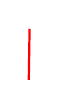
\begin{tikzpicture}\draw[red,line width=0.8pt] (0,0)--(0.01,0.65);\end{tikzpicture}} Réciproque vraie si $E$ et $F$ de dimension infinie. \uline{En tous cas}, $L_N(E,F)$ réfl. $\Longleftrightarrow L^N(E,F)$ réflexif $\Longleftrightarrow\ldots$

\uline{Corollaire 3} Si $1<p<+\infty$, alors $L^p(E,F)$ est un espace réflexif ayant pour dual $L^{p'}(F,E)$

\uline{Prop} Si $N,N',N''$ sont des normes de Schatten telles que $N(xy)\leq N'(x)N'(y)$, alors $u\in L^{N'}(E,F)$, $v\in L^{N''}(F,G)$ implique $vu\in L^N(E,F)$, \inserted{et $N(vu)\leq N'(u)N''(v)$ \uline{Corollaire}} Si \uline{un des \deleted{\unsure{soit}} $N',N''$ est mis en} bas, on peut faire de $=$ avec l'autre. \margin{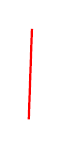
\begin{tikzpicture}\draw[red,line width=0.8pt] (0,0)--(0.04,1.15);\end{tikzpicture}}

(\deleted{par transposition, on se ramène \unsure{au deuxième} \illegible{2}, en} \deleted{prenant $N'''=N^\circ$,} Par le deuxième th. de convexité si $v$ et $u$ sont \deleted{\unsure{là par contraction}, on} \deleted{à prouver que si $N_1(xyz)\leq N'(x)N''(y)N'''(z)$, alors} \unsure{cpts.|cpcts.} On s'y ramène facilement, en notant que \deleted{on a $N_1(wvu)\leq N'(u)N''(v)N'''(w)$.}

\[
N(u)=\lim N(\underline{pu}\deleted{\unsure{p|q}})=\lim_p N(pup)=\lim_p N(\unsure{up|u_p})
\]

$p$ projecteur orth. de rang fini, \uline{variant} en filtrant croissant. (\unsure{Car|Donc} $N(pvup)=N((pv)(up))\leq N''(pv)N^{\unsure{''|'}}(up)\leq N''(v)N^{\unsure{\circ|'}}(u)$). Enfin, rappelons

\uline{Prop} $N((\lambda_i u))\leq N(u)$

\uline{Prop} Caractérisation des espaces de Schatten.

\margin{104}


\scanpage{104}

\uline{Théorème} \textcircled{1} Soit $N$ une norme de Schatten sur $R^{(\underline N)}$, \deleted{Soient $E$ et $F$}\inserted{pour tout couple $(E,F)$ de} deux espaces de \deleted{Banach}\inserted{Hilbert}, \deleted{posons}\inserted{et} pour $u\in L_0(E,F)$, posons

\margin{\begin{tikzpicture}[x=1cm,y=1cm]\draw[line width=.2pt] (0,0)--(.03,-.9);\end{tikzpicture}}
\[
N(u)=N((\rho_i(u)))\tag*{(18)}
\]

et pour $u\in L(E,F)$

\margin{\begin{tikzpicture}[x=1cm,y=1cm]\draw[line width=.2pt] (0,0)--(.12,-3.3);\end{tikzpicture}}
\[
N(u)=\underset{\substack{v\in F'\otimes E\\N^\circ(u)\leq 1}}{\operatorname{Sup}}|\operatorname{Tr}vu|\tag*{(19)}
\]

Cette deuxième expression coïncide avec la précédente sur $L_0(E,F)$. Soit $L^N(E,F)$ le sous-espace de $L(E,F)$ formé des $u$ tels que $N(u)<+\infty$, alors $N$ est une norme sur $L^N(E,F)$, qui en fait un espace de Banach. \deleted{L'adhérence \inserted{$L_N(E,F)$} de $E'\otimes F$ dans cet \unsure{espace est} l'espace des $u\in L_0(E,F)$ tels que} \inserted{Si $u\in L_0(E,F)$, alors on} a $u\in L^N(E,F)$ si et seulement si $(\rho_i(u))\in\ell^N$, et alors on a (18). \deleted{\unsure{N}} L'adhérence \inserted{$L_N(E,F)$} de $E'\otimes F$ dans $L^N(E,F)$ est l'ensemble des op. \deleted{\unsure{cpts}} $u\in L_0(E,F)$ tels que $(\rho_i(u))\in\ell_N$.

\margin{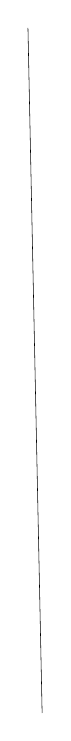
\begin{tikzpicture}[x=1cm,y=1cm]\draw[line width=.2pt] (0,0)--(.18,-8.7);\end{tikzpicture}}
\textcircled{2} On a

\[
\boxed{N(u)=N(u^*)}\boxed{\deleted{\unsure{N(u)}}}\tag*{\textcircled{20}}
\]

et par suite $u\in L^N(E,F)\mathrel{\textcolor{red}{\underline{\textcolor{black}{=}}}}u^*\in L^N(F,E)$
\margin{\deleted{\unsure{$\Longleftrightarrow u\in L^N(E,F)$|sur $L^N(E,F)$}}\quad\textcolor{red}{?}}
\inserted{de $=$} $u\in L_N^c(E,F)\mathrel{\textcolor{red}{\underline{\textcolor{black}{\Longleftrightarrow}}}}u^*\in L_N(F,E)$. On a

\[
\begin{aligned}
N(uv)&\leq\lVert u\rVert N(v)\\
N(uv)&\leq\lVert v\rVert N(u)
\end{aligned}\tag*{\textcircled{21}}
\]

si $u\in L(E,F)$, $v\in L(F,G)$. \deleted{\unsure{Donc}} En composant à gauche ou à droite un op. \deleted{$\in L^N($} du type $\ell^N$ (resp$^t$ $\ell_N$) avec un opérateur \deleted{de type} \textcolor{red}{\uline{\textcolor{black}{continu}}}, on obtient un op. du type $\ell^N$ (resp.t $\ell_N$).
\margin{\begin{tikzpicture}[x=1cm,y=1cm,line cap=round]\draw[red!70!brown,line width=.4pt] (0,.56)..controls(.015,.47)and(.045,.40)..(.035,.36)..controls(.025,.33)and(.07,.32)..(.075,.35);\draw[red!50!brown,line width=.25pt] (.075,.35)..controls(.16,.37)and(.16,.16)..(.11,.09)..controls(.07,.07)and(.11,.02)..(.10,0)..controls(.11,.04)and(.16,.10)..(.16,.13);\end{tikzpicture}}
\inserted{$N(u)$ est fonction croissante sur l'ens. des hermitiens positifs dans $L_0(E)$.}

\textcircled{3} \deleted{\textcircled{4}} Si $N,N',N''$ sont \deleted{\unsure{deux|une}}\inserted{des} normes de Schatten telles que

\[
\text{\unsure{p.|q.}}\qquad\boxed{N(xy)\leq N'(x)N'(y)}\tag*{\textcircled{22}}
\]

pour $x,y\in R^{(\underline N)}$, alors on a, pour $u\in L(E,F)$, $v\in L(F,G)$,

\[
N(vu)\leq \unsure{N'(v)|N'v)}N''(u)\tag*{\textcircled{23}}
\]

donc si $u\in L^{N'}(E,F)$, $v\in L^{N''}(E,F)$, alors $vu\in L^N(E,F)$, et si on a \inserted{de plus} $u\in L_{N'}(E,F)$ ou $v\in L_{N''}^{\unsure{\deleted{N}|*}}(E,F)$, on aura $=$ $vu\in L_N(E,F)$, -- En particulier, on aura, pour $u\in L(E,F)$, $v\in L(F,\unsure{G|E})$

\[
\lVert vu\rVert_1\leq N(u)N^\circ(v)\tag*{\textcircled{24}}
\]

donc si $u\in L^N(E,F)$, $v\in L^{N^\circ}(F,\unsure{G|E})$, on a $vu\in L^1(E,\unsure{E|G})$, et

\[
|\operatorname{Tr}vu|\leq N(u)N^\circ(v).\tag*{\textcircled{25}}
\]

\margin{105}



\scanpage{105}

\margin{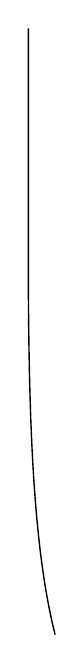
\begin{tikzpicture}\draw[line width=0.5pt] (0,7.7)--(0,4.4).. controls (0.01,2.7) and (0.06,1.1) .. (0.34,0);\end{tikzpicture}}
\textcircled{4} Par l'accouplement \deleted{\unsure{de}}

\[
\langle u,v\rangle=\operatorname{Tr}vu\tag*{\textcircled{26}}
\]

le dual de $L_N(E,F)$ s'identifie à $L^{N^\circ}(F,E)$. Si $E$ et $F$ sont de dimension infinies, \deleted{\unsure{les espaces suivants|les deux conditions} $L_N(E,F)$} \inserted{alors} conditions suivantes sont équivalentes\,: a) $L_N(E,F)$ est réflexif \deleted{$L_N(E,F)=L^N(E,F)$ et $L_{N^\circ}(F,E)=L^{N^\circ}(\unsure{F|F,E})$} b) $L^N(E,F)$ est réflexif c) $\ell^{\deleted{\unsure{\ell|N}}}_{N}$ est réflexif \deleted{\unsure{f),}} d) $\ell_{N'}$ est réflexif. \deleted{\unsure{c'est et seulement si}, \unsure{$\ell$} \unsure{équiv$^{\mathrm{tes}}$ de ces propositions à}\,: d) $\ell^N$ est réflexif. -- e) $\ell_{N^\circ}$ est réflexif et \unsure{enfin} f) $\ell^{N^\circ}$ est réflexif)} \deleted{\unsure{alors}} d) $L_N(E,F)=L^N(E,F)$ et $\begin{aligned}&L_{N^\circ}(F,E)=L^{N^\circ}(F,E)\\[-0.5ex]&\quad\text{\deleted{\unsure{et}}}\end{aligned}$

\textcircled{5} \deleted{\unsure{Remarquons|Remarque}} Soit $u\in L_0(E,F)$, \deleted{si $u\in L^N(E,\unsure{F|E})$\unsure{,} \unsure{alors} \unsure{Alors} $(\lambda_i(u))\in\ell^N$,} \inserted{Alors}

\[
N((\lambda_i(u)))\leq\deleted{N(\unsure{(\rho_i(u))|(\rho_i u)})}N(u)\tag*{(27)}
\]

Si $u\in L^N(E,F)$, \deleted{alors (resp$^t$ $L_N(E,E)$)} alors, $(\lambda_i(u))\in\deleted{\unsure{\ell_N|L^N\unsure{,}|\ell^N}}\ell^N$ \deleted{(resp$^t$ $\ell_N$)}

Tout est démontré, sauf 4. \deleted{\unsure{et}} et 5. Pour 4, on note\,: si $E$ et $F$ sont de dimension infinie, alors $\ell^N$ \inserted{(resp$^t$ $\ell_N$)} est isométrique à un sous-espace vectoriel normé de $L^N(E,F)$ (resp$^t$ $L_N(E,F)$. (\textcolor{red}{\uline{\textcolor{black}{prendre}}} $(e_i)$, $(f_i)$ systèmes orthonormaux infinis, et $(\lambda_i)\to\sum\lambda_i\bar e_i\otimes f_i$ de $\ell^N$ dans $L^N(E,F)$). \deleted{Donc}

Si $L^N_{\deleted{\unsure{0|N}}}(E,F)$ est réflexif, $L_N(E,F)$ est réflexif, et alors aussi $\ell_N$ est réflexif, \deleted{\unsure{donc}}\inserted{\unsure{Celà|ce q.} implique} (voir --) $\ell_N=\ell^N$, $\ell_{N^\circ}=\ell^{N^\circ}$, donc $L^N(E,F)=L_N(E,F)$ (car on \deleted{\unsure{peut supposer}}\inserted{aura} exigé $N\unsure{\not\simeq|\neq}N_\infty$), donc $L^N(E,F)$ sera réflexif, d'où l'équivalence a), b), c).

\margin{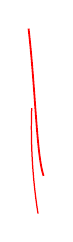
\begin{tikzpicture}\draw[red,line width=0.65pt] (0,2.35).. controls (0.09,1.55) and (0.10,0.75) .. (0.19,0.48);\draw[red,line width=0.45pt] (0.04,1.34).. controls (0.02,0.79) and (0.07,0.31) .. (0.12,0);\end{tikzpicture}}
Et le fait que cela implique d) (d'abord la première assertion, pour la seconde on $\ell_{N^\circ}$ sera aussi réflexif). Enfin d implique \deleted{$\ell_N=\ell^N$ et $\ell_{N^\circ}=\ell^{N^\circ}$ (voir \unsure{théorème précédent|th. précédent}) donc $\ell_N$ réflexif (\unsure{toujours|voir --})} \inserted{que le dual de $L_N(E,F)$ est $L_{N^\circ}(F,E)$,} dont le dual est $L_N(E,F)$, donc $L_N(E,R)$ est réflexif.

\textcircled{5} (27) Est le corollaire 5 du 1. th. de convexité \deleted{\unsure{Résulte aussitôt du|résulte immédiatement}}
\margin{106}


\scanpage{107}

Décomposition en facteurs des fonctions entières.

\margin{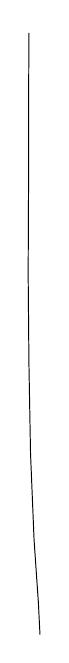
\begin{tikzpicture}[x=0.005cm,y=-0.005cm,baseline={(0,0)}]
\draw[line width=0.35pt] (19,13) -- (18,210) -- (18,400) -- (17,625) -- (19,855) -- (23,1080) -- (32,1300) -- (43,1460) -- (47,1540);
\end{tikzpicture}}
\uline{Théorème 1} (Weierstrass) Soit $f(z)$ fonction entière, $(a_n)$ la suite de ses zéros, rangés par ordre \unsure{en|de} modules croissants. Supposons $f(0)\ne0$. Il est possible de trouver une suite croissante de nombres entiers $\geq0$ $p_n$, et une fonction entière $g(z)$, tels que l'on ait

\[
 f(z)=e^{g(z)}\prod_n\left(1-\frac{z}{a_n}\right)e^{\frac{z}{a_n}+\frac{z^2}{2a_n^2}\unsure{+}\mathord{\cdot}\mathord{\cdot}\frac{z^{p_n}}{p_n a_n^{p_n}}} \tag*{(1)}
\]

le produit étant uniformément absolument convergent quand $z$ parcourt n'importe quelle région bornée. Si \deleted{de plus} \inserted{une suite d'entiers} $p_n$ vérifie

\[
 \sum\left|\frac{r}{a_n}\right|^{(p_n+1)}<+\infty\qquad\text{quel que soit }r,
\]

alors on peut employer cette suite dans l'expression \uline{1}. En particulier, supposons $k$ un entier tel que $\sum\frac{1}{|a_n|^{k+1}}<+\infty$, alors on peut prendre $p_n\deleted{\unsure{=|k}}\unsure{=}p$ pour \deleted{tout} $n$, avec $p\leq k$ d'où

\[
 f(z)=e^{g(z)}\prod_n\left(1-\frac{z}{a_n}\right)e^{\frac{z}{a_n}+\unsure{-|\cdots}+\frac{z^k}{ka_n^k}} \tag*{(2)}
\]

\margin{108}


\scanpage{108}

\uline{Genre d'une fonction entière}

Il arrive que l'on ait $\sum\frac{1}{|a_n|^{k+1}}<+\infty$ pour quelque $k$, (soit $k$ le plus petit entier qui y satisfasse) et de plus que dans la repré-\newline sentation (2), $g(z)$ soit un polynôme -- d'ailleurs déterminé à une constante près.

Soit $r$ son degré, le plus \deleted{petit} \inserted{grand} des nombres $r,k$ s'appelle le genre de $f(z)$.
\inserted{C'est un nb \uline{entier} $\geq 0$.}

Donc si $f(z)$ est de genre $\leq r$, alors on a la formule
\[
f(z)=e^{\alpha_0+\alpha_1 z\mathord{\cdot}\mathord{-}+\alpha_n z^n}\prod_n\left(1-\frac{z}{a_n}\right)e^{\frac{z}{a_n}+\mathord{-}\mathord{\cdot}\frac{z^{\unsure{n|r}}}{r a_n}}\tag*{(3)}
\]

Dire que $f(z)$ est de genre zéro, signifie que $f(z)$ est de la forme
\[
\begin{aligned}\vphantom{f(z)}\\[-2pt]\text{avec}\quad\end{aligned}
\left\{\begin{aligned}
f(z)&=\mathrm c^{\mathrm{te}}\times\prod_n\left(1-\frac{z}{a_n}\right)\unsure{.|,}\\[-2pt]
\sum_n\frac{1}{|a_n|}&<+\infty
\end{aligned}\right.\tag*{(4)}
\]

\uline{Ordre d'une fonction entière} \quad Posons $M(r)=\mathop{\rm Sup}_{z\unsure{=|\leq}r}|f(z)|$

Puis $\rho=\overline{\lim}\frac{\log\log M(r)}{\substack{\deleted{\unsure{z}}\\\inserted{\log r}}}$ \quad $(0\leq\rho\leq+\infty)$, $\rho$ est dit l'ordre de $f(z)$, et $f(z)$ est dite d'ordre
\par\noindent\hspace{2cm}\unsure{$=$}\par\noindent
fini si $\rho<+\infty$. Cela signifie qu'il existe $k>0$ tel que $|f(z)|\leq e^{\unsure{(z\vert^k)|(\lvert z\rvert^k)}}$. Alors $\rho$ est la \deleted{\unsure{plus petit nombre|plus petite valeur}} \inserted{borne inférieure des} $\sigma>0$ tels que

\margin{109}


\scanpage{109}
\deleted{\unsure{soit|ait}} \inserted{l'on ait} $M(r)\leq e^{(r^\sigma)}$ pour $r$ assez grand.

\margin{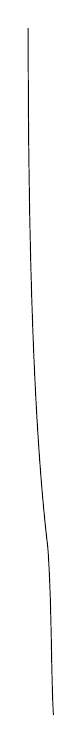
\begin{tikzpicture}[x=0.1mm,y=0.1mm,baseline=(current bounding box.north)]
\draw[line width=0.35pt] (0,0) .. controls (0,-260) and (6,-500) .. (25,-660) .. controls (30,-730) and (29,-815) .. (32,-872);
\end{tikzpicture}}
\uline{Théorème 2} (Hadamard-Borel) Si l'ordre $\rho$ de $f(z)$
est fini, alors pour \deleted{tout} $\varepsilon>0$, la série
\[
\sum{}'\frac{1}{|a_n|^{\rho+\varepsilon}}<+\infty \tag*{(5)}
\]
($'$ indique
qu'on ne somme pas sur les racines nulles)

De plus, on a alors (en supposant $f(0)\ne0$)
\[
f(z)=e^{P(z)}\prod_n\left(1-\frac{z}{a_n}\right)e^{\frac{z}{a_n}+\mathord{-}+\frac{z^p}{p a_n^p}}
\]
où $p\leq\rho$, et $P(z)$ est \deleted{\unsure{un polynôme}} \inserted{un polynôme}
de degré $\leq\rho$ : en d'autres termes, on
a \qquad genre de $f$ $\leq\rho=$ ordre de $f$

\uline{Corollaire} \quad Si $\rho<1$, i.e s'il existe un $0<\mu<1$
tel que $M(r)\leq e^{(r^\mu)}$ pour $r$ assez grand,
alors $f(z)$ est de genre zéro :
\[
f(z)=\mathrm{c}^{\mathrm{te}}\mathbin{\times}\prod_n\left(1-\frac{z}{a_n}\right)\deleted{\unsure{e^{z/a_n}}}
\]

\uline{Remarque}. \quad Il est très facile de se convaincre
que \qquad ordre de $f$ $\leq$ genre de $f+1$. Donc, si $\omega$ et
$g$ sont respectivement le genre et l'ordre, on a
\begin{center}
\makebox[0pt][l]{\raisebox{-2mm}{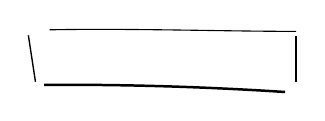
\begin{tikzpicture}[x=1mm,y=1mm]
\draw[line width=0.4pt] (2.7,7.2) .. controls (13,7.4) and (25,7.0) .. (34,7.0);
\draw[line width=0.5pt] (0,6.5) -- (0.9,0.6);
\draw[line width=0.45pt] (34,6.4) -- (34,0.6);
\draw[line width=0.9pt] (2,0.2) .. controls (14,0.3) and (25,-0.2) .. (32.6,-0.7);
\end{tikzpicture}}}\makebox[34mm]{\(\omega-1\leq g\leq\omega\)}
\end{center}

Comme $\gamma$ est entier, il en résulte que $\gamma$
est connu dès que $\omega$ l'est, sauf si $\omega$ est
entier. En ce cas, on peut avoir $p=\omega$, ou
$\gamma=\omega-1$
\margin{110}


\scanpage{111}

\uline{Proposition} \quad Soit $f(z)$ une fonction entière \deleted{\unsure{satisfaisant}} \deleted{\unsure{majorée}} \inserted{dont} \deleted{\unsure{avec|dont}} \inserted{les} coefficients sont majorés en module par ceux d'une fonction de genre $0$ $h(z)$. Si de plus les racines non nulles $z_i$ de $f(z)$ sont telles que $\sum\frac{1}{|z_i|}<+\infty$, $f(z)$ est de genre zéro.

\deleted{En effet, $h(z)$ étant d'}

Démonstration. On peut supposer que $h(z)$ est de la forme $k^{\mathrm{te}}\times\sum_{i=1}^{\infty}(1+\alpha_i z)$, où les $\alpha_i$ sont $>0$, et $\sum\alpha_i<+\infty$. Comme $h(z)$ est d'\uline{ordre} $\leq1$, il en est de $=$ de $f(z)$, donc on aura,
\[
f(z)=e^{\alpha+\beta z}z^m\prod_i\left(1-\frac{z}{z_i}\right)
\]

Il faut montrer que $\beta=0$. On peut supposer pour simplifier $\beta>0$, sinon on remplacerait $f(z)$ par $f(\Theta z)$, avec $\Theta=\beta/|\beta|$. On a alors $\displaystyle |f(z)|=\unsure{K_1^{\mathrm{te}}|K^{\mathrm{te}}}\times e^{\beta x}|z|^m\prod\left|1-\frac{z}{z_i}\right|$\unsure{.}

D'autre part, on sait que \deleted{\unsure{si une}} \inserted{toute} fonction de genre zéro, telle $h(z)$, admet une majoration de la forme $|h(z)|\leq\mathrm C^{\mathrm{te}}\times e^{\varepsilon|z|}$, où on peut prendre $\varepsilon$ arbitraire. \deleted{Si alors on prend $\varepsilon\unsure{<|\leq}\beta$, on aura}
\[
\deleted{\deleted{|f(z)|\leq}|z|^m\prod\left|1-\frac{z}{z_i}\right|\leq\unsure{K|C}e^{\varepsilon|z|}}
\]
\deleted{\unsure{avec|pour|tout} $z$}
\margin{112}


\scanpage{112}
Notons que si $-\theta\leq\arg z\leq+\theta$, où $\theta$ est
un angle arbitraire que nous prendrons une
fois pour toutes entre $\frac{\pi}{3}$ et $\pi$, on
aura $x\geq c|z|$, où $c$ est une
constante $>0$, d'où \deleted{$f(z)\geq$}
\figure{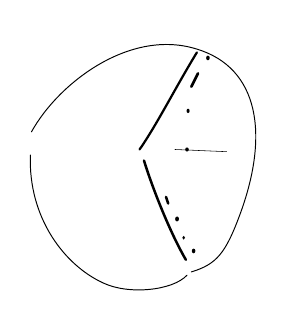
\begin{tikzpicture}[x=.014cm,y=-.014cm,line cap=round,line join=round]
\draw[line width=.35pt] (14,95) .. controls (39,50) and (104,1) .. (164,20) .. controls (220,37) and (230,97) .. (203,170) .. controls (190,205) and (182,215) .. (159,222);
\draw[line width=.35pt] (13,116) .. controls (11,173) and (44,216) .. (79,232) .. controls (102,243) and (142,239) .. (155,225);
\draw[line width=.8pt] (112,111) .. controls (128,88) and (145,54) .. (164,23);
\draw[line width=.9pt] (116,121) .. controls (124,147) and (140,187) .. (154,211);
\fill (174,28) ellipse [x radius=.65pt,y radius=.85pt];
\draw[line width=1pt] (165,42)--(159,54);
\fill (156,76) ellipse [x radius=.55pt,y radius=.8pt];
\draw[line width=.9pt] (136,154)--(138,160);
\fill (146,174) ellipse [x radius=.7pt,y radius=.9pt];
\fill (152,191) ellipse [x radius=.5pt,y radius=.7pt];
\fill (161,203) ellipse [x radius=.65pt,y radius=.85pt];
\draw[line width=.2pt] (144,111)--(191,113);
\fill (155,111) ellipse [x radius=.65pt,y radius=.75pt];
\end{tikzpicture}}
\[ |f(z)|\geq e^{c|z|}|z|^m\prod_i\left|1-\frac z{z_i}\right|\qquad\text{qnd }-\theta\leq\arg z\leq+\theta \]

D'autre part on a $|f(z)|\leq|h(z)|\leq \mathrm c^{\mathrm{te}}\times e^{\varepsilon|z|}$
d'où, en supposant qu'on ait choisi $\varepsilon<c$
\[ |z|^m\prod_i\left|1-\frac{z}{z_i}\right|\leq k e^{-\alpha|z|} \]
où $\alpha>0$, dès que $-\theta\leq\arg z\leq+\theta$.

Posons $g(z)=z^m\prod_i(1-\frac z{z_i})$, notre formule
s'écrit \quad \uline{$|g(z)|\leq ke^{-\alpha|z|}$} \quad si $-\theta\leq\arg z\leq+\theta$

Montrons qu'une \deleted{telle} inégalité n'est possible
pour une fonction $g$ de genre zéro que si elle
est \deleted{\unsure{identique}} \inserted{constante}. On a en effet aussi, $g$ étant de genre
zéro \qquad $|g(z)|\leq k'e^{\frac{\alpha}{3}|z|}$ \qquad pour l'ensemble
Posons $\omega=e^{\frac{2i\pi}{3}}$, et $G(z)=g(z)g(\omega z)g(\omega^{\unsure{3|2}}z)$
C'est une fonction entière, et on vérifie
aussitôt que, \uline{quel que soit $z$}, on a
\[ |G(z)|\leq(ke^{-\alpha|z|})(k'e^{\frac{\alpha}{3}|z|})(k'e^{\frac{\alpha}{3}|z|})=k''e^{-\frac{\alpha}{3}|z|} \]
\noindent\quad\unsure{!!}

$G(z)$ serait donc bornée, donc une constante.
Mais $G(z)=z^{\unsure{-3m|3m}}\prod_i\left(1-\frac{z^3}{z_i^3}\right)$, il
\margin{faudra que l'ens. d'indices $i$ soit vide, et $m=0$, donc
que $g(z)$ soit une constante. Cel. signifie
que $f(z)=\mathrm C^{\mathrm{te}}e^{\beta z}$, ce qui est incompatible
avec $|f(z)|\leq|\deleted{\unsure{g}}h(z)|\leq \mathrm c^{\mathrm{te}}e^{\varepsilon|z|}$}
\margin{113}


\scanpage{113}
Soit $(\alpha_n)$ une suite \uline{décroissante} \inserted{et convergeant vers zéro} de nombres
positifs. Soit $\rho$ la borne inférieure des nombres
\deleted{positifs} $s>0$ tels que $(\alpha_n)$ soit majorée par
un multiple de la série $\left(\frac{1}{n^{1/s}}\right)$ (et $+\infty$
si un tel $s$ n'existe pas) et soit $\sigma$ la
borne inférieure des nombres $s>0$, tels que
$\sum_n\alpha_n^s<+\infty$. (et $+\infty$ si un tel $s$ n'existe pas)

On a aussi $\frac1\rho\deleted{\unsure{\leq}}\inserted{=}\limsup_n\unsure{:}\frac{\log(1/\alpha_n)}{\log n}$. \deleted{$\rho$ et $\sigma$
sont \unsure{resp\textsuperscript{t}} les bornes inf. d'ensembles
A et B.} -- Le critère de Riemann affirme
que \deleted{$\unsure{\rho\leq|\rho\leq\sigma}$} $\sigma\leq\rho$. Mais on a aussi $\rho\leq\sigma$,
car \unsure{on a le|en effet}

\uline{Lemme} \quad Si $s>0$ est tel que $\sum_n\alpha_n^s<+\infty$
alors \inserted{$\geq$} \deleted{la suite $(\alpha_n)$ est majorée par un
multiple de la suite $\left(\frac1{n^{1/s}}\right)$} \inserted{$\alpha_n=o\left(\frac1{n^{1/s}}\right)$}. ($\alpha_n$ étant décroissant !)

Démonstration. On se ramène au cas où $s=1$
(en posant $B_n=\alpha_n^s$) \inserted{et à prouver qu'il est impossible que} \deleted{\unsure{sup}} pour une suite
strictement croissante d'entiers $n_i$, on \deleted{avait} ait
$\alpha_{n_i}\geq\frac1{n_i}$ ; \inserted{en effet, alors} on aurait \quad $\alpha_{n_{i-1}+1}+\alpha_{n_{i-1}+2}\unsure{+|\mathord{-}}\,\mathord{-}+\alpha_{\unsure{n_i|n}}\geq\frac{n_i-n_{i-1}}{n_i}$
soit $\varepsilon_i$ ce second membre, $\sum\varepsilon_i$ est \unsure{donc}
convergente, et on a $n_i(1-\varepsilon_i)=n_{i-1}$, d'où $n_i=\frac{n_{i-1}}{1-\varepsilon_i}$
$\displaystyle =\frac{n_{i-2}}{(1-\varepsilon_i)(1-\varepsilon_{i-1})}\mathord{-}\,\mathord{-}\,\mathord{-}\,\mathord{-}=\frac1{(1-\varepsilon_{\unsure{1|i|0}})\unsure{\mathord{.}\,\mathord{-}|\ldots}(1-\varepsilon_{\unsure{n|i|m}})}\leq\frac1{\prod_1^\infty(1-\varepsilon_k)}$, la suite
des $n_i$ est donc majorée, et s'arrête donc.
\margin{114}


\scanpage{114}
\uline{Supposons} maintenant que l'on ait $\sum\alpha_i<+\infty$,
posons $f(z)=\prod_1^\infty(1+\alpha_i z)$. Alors $\rho$ est aussi
l'ordre de la fonction entière, i.e
\[ \rho=\limsup_{0<r\to\infty}\frac{\log(\log f(r))}{\log r} \]

En effet, on sait que $\rho$ est $\leq$ ordre de la
fonction $f(z)$, \deleted{\unsure{et}} \unsure{montrons|démontrons} le contraire. On est
\uline{ramené} à montrer que \unsure{.|:} \deleted{le produit} dans le
cas où on a $\alpha_n=\frac1{n^\beta}$, on a
$\displaystyle \limsup_{0<r\to\infty}\frac{\log\log f(r)}{\log r}\leq\frac1\beta$ \quad (en somme on a en fait $=\frac1\beta$)

En effet, on a
\[ f(r)=\prod_1^\nu\left(1+\frac1{n^\beta}r\right)\prod_{\nu+1}^{\infty}\left(1+\frac1{n^\beta}r\right) \]
le deuxième facteur est $\leq e^{R(\nu)r}$
avec $\displaystyle R(\nu)=\sum_{\nu+1}^\infty\frac1{n^\beta}\leq\int_\nu^\infty\frac{du}{x^\beta}=\frac1{\beta-1}\frac1{\nu^{\beta-1}}$
Prenons $\nu$ tel que $r\unsure{\cdot}\frac1{\nu^{\beta-1}}\leq r^{\frac1\beta}$, i.e $\nu\geq r^{\frac1\beta}$
de façon précise, $\nu=[r^{\frac1\beta}]+1$. Alors, $e^{R(\nu)r}$
sera une \uline{fonction de $r$} d'ordre $\leq\frac1\beta$\unsure{;|.} Il
suffit de le vérifier pour le produit $\prod_1^\nu(1+\frac1{n^\beta}r)$
$\leq(1+r)^\nu=e^{\nu\log(1+r)}$, qui est manifestement
d'ordre $\leq\frac1\beta$.

Rappelons que si on pose $f(\unsure{r|z})=\sum a_n z^n$,
\deleted{\unsure{dans|donc}} et $\unsure{B|D}(r)=\mathop{\rm Sup}_n(a_n r^n)$, alors on
a aussi \qquad ordre \unsure{a|de} $f=\limsup_{r\to\infty}\frac{\log\log B(r)}{\log r}$
\margin{115}


\scanpage{115}
Soit $f(z)=\prod_1^\infty(1+\lambda_i z)$ une fonction entière
de \uline{genre} $1$, posons $\alpha_i=|\lambda_i|$, $F(z)=\prod_{\unsure{1|i}}^\infty(1+\alpha_i z)$.
Alors \uline{$f$ et $F$ ont $=$ ordre} (qui s'exprime donc
aussi en fonction de la suite des $|\alpha_i|$). En effet,
l'ordre de $f\leq$ ordre de $F$ (évident). D'autre
part, ordre de $F=$ ordre de la suite des $|\alpha_i|$
(voir ci-dessus) $\leq$ ordre de $f$ (th. de Hadamard)
\begin{center}\rule{1.5cm}{0.4pt}\end{center}

On peut parler de l'ordre d'un ensemble \inserted{dénombrable} de
nombres complexes, \deleted{\unsure{indépendamment de}} \inserted{$=$ \unsure{non} compris en suite :}
on prend la borne inf. des $s>0$ tels que
$\sum|z_i|^s<+\infty$. Suite à décroissance rapide $=$
d'ordre zéro.

Ordre d'une suite dans un espace de Banach,
ou de Fréchet. (deux définitions, suivant qu'on
prend sommabilité forte, ou sommabilité absolue)

Ordre d'une partie bornée (\deleted{plus petit} \inserted{borne inférieure} des
$s>0$ tels que la partie soit contenue dans l'envelop-\newline
pe convexe cerclée fermée d'une suite d'ordre $s$)
\margin{116}


\scanpage{116}
Soit $(r_\nu)$ suite croissante de nombres \deleted{\unsure{positifs}} $>0$, $\to\infty$
soit $n(r)$ le nombre des indices $\nu$ tels que
$r_\nu\leq r$, on a, pour $0\leq a\leq b<+\infty$, et $\alpha>0$
\[ \hbox{\begingroup\setbox0=\hbox{$\displaystyle \sum_{\substack{\nu\\(a<r_\nu<b)}}\frac1{r_\nu^\alpha}=\left(\frac{n(b-0)}{b^\alpha}-\frac{n(a+0)}{a^\alpha}\right)+\alpha\int_a^b\frac{n(r)\,dr}{r^{\alpha+1}}$}\kern5pt\rlap{\tikz[baseline=0pt]{\draw[line width=.35pt] (-1pt,\the\dimexpr\ht0+4pt\relax)--(\the\dimexpr\wd0+7pt\relax,\the\dimexpr\ht0+4pt\relax);\draw[line width=.35pt] (-5pt,\the\dimexpr\ht0+1pt\relax)--(-5pt,\the\dimexpr-\dp0-1pt\relax);\draw[line width=.45pt] (\the\dimexpr\wd0+5pt\relax,\the\dimexpr\ht0+1pt\relax)--(\the\dimexpr\wd0+5pt\relax,\the\dimexpr-\dp0-1pt\relax);\draw[line width=.4pt] (-1pt,\the\dimexpr-\dp0-4pt\relax)--(\the\dimexpr\wd0+5pt\relax,\the\dimexpr-\dp0-4pt\relax);}}\copy0\kern7pt\endgroup}\tag*{(1)} \]
(car le premier membre est égal à : $\int_{\unsure{r_0|a_0}}^b r^{-\alpha}\,dn(r)$,
et on intègre par parties)

\uline{Proposition} \quad $\displaystyle \sum_\nu\frac1{r_\nu^\alpha}<+\infty\ \Longleftrightarrow\ \int_0^\infty\frac{n(r)\,dr}{r^{\alpha+1}}\leq+\infty$
\margin{\tikz[x=1pt,y=1pt]{\draw[line width=.35pt] (0,0)--(.4,-68);}}
alors $\frac{n(r)}{r^\alpha}\to0$ pour $r\to\infty$, et on a
\[ \hbox{\begingroup\setbox0=\hbox{$\displaystyle \sum_{\substack{\nu\\(r_\nu>a)}}\frac1{r_\nu}=-\frac{n(a+0)}{a^\alpha}+\alpha\int_a^\infty\frac{n(r)\,dr}{r^{\alpha+1}}$}\kern5pt\rlap{\tikz[baseline=0pt]{\draw[line width=.35pt] (-1pt,\the\dimexpr\ht0+4pt\relax)--(\the\dimexpr\wd0+7pt\relax,\the\dimexpr\ht0+4pt\relax);\draw[line width=.35pt] (-5pt,\the\dimexpr\ht0+1pt\relax)--(-5pt,\the\dimexpr-\dp0-1pt\relax);\draw[line width=.45pt] (\the\dimexpr\wd0+5pt\relax,\the\dimexpr\ht0+1pt\relax)--(\the\dimexpr\wd0+5pt\relax,\the\dimexpr-\dp0-1pt\relax);\draw[line width=.4pt] (2pt,\the\dimexpr-\dp0-4pt\relax)--(\the\dimexpr\wd0+5pt\relax,\the\dimexpr-\dp0-4pt\relax);}}\copy0\kern7pt\endgroup}\tag*{(1)} \]

$\leftarrow$
\deleted{\unsure{si} $\sum_\nu\frac1{r_\nu^\alpha}<+\infty$, \unsure{on a} $\frac{n(r)}{r^\alpha}\leq M$ pour \deleted{\unsure{tout}} $r$
où $M=$ \unsure{constante}}
En effet, (1) s'écrit, pour $a=0$, \deleted{\unsure{comme|donc}}
\[ \sum_{r_\nu<b}\frac1{r_\nu^{\unsure{\nu|\alpha}}}=\frac{n(b-0)}{b^\alpha}+\alpha\int_0^b\frac{n(r)\,dr}{r^{\alpha+1}}\tag*{\textcircled{\scriptsize 1 bis}} \]
d'où suit que si \deleted{\unsure{pour un|pour} $b$} $\sum_\nu\frac1{r_\nu^\alpha}$ est
convergente, il en est de $=$ de $\int_0^\infty\frac{n(r)\,dr}{r^{\alpha+1}}$
Réciproquement, si $\int_{\unsure{0}}^\infty\frac{n(r)\,dr}{r^{\alpha+1}}<+\infty$ alors il
existe $M>0$ et une suite croiss. de $b_i\to\infty$
de nbs tels que $\frac{n(b_i)}{b_i^\alpha}\leq M$ ; \unsure{p.} on a donc
$\displaystyle \sum_{r_\nu<b_i}\frac1{r_\nu^\alpha}\leq M+\alpha\int_0^\infty\frac{n(r)\,dr}{r^{\alpha+1}}$, d'où $\displaystyle \hbox{\begingroup\setbox0=\hbox{$\displaystyle\sum_{\unsure{\nu|i}}\frac1{r_{\unsure{\nu|i}}^\alpha}$}\rlap{\raisebox{\dimexpr-\dp0-2pt\relax}{\tikz[baseline=0pt,x=1pt,y=1pt]{\draw[line width=.4pt] (0,3)--(0,0)--(\the\wd0,0)--(\the\wd0,3);}}}\copy0\endgroup}<+\infty$.
\margin{117}


\scanpage{117}
Montrons qu'alors $\frac{n(r)}{r^\alpha}\to0$ ; si en effet on avait
$\frac{n(b_i)}{b_i^\alpha}>\varepsilon$ pour des $b_i\to+\infty$, on aurait
$n(b_i)-n(b_{i-1})\geq\varepsilon\lambda_i^\alpha-M\lambda_{i-1}^\alpha$ d'où
\[
\sum_{\substack{\nu\\b_{i-1}<r_\nu\leq b_i}}r_\nu^{-\alpha}\geq\big(n(b_i)-n(b_{i-1})\big)\lambda_i^{-\alpha}\geq\varepsilon-M\left(\frac{\lambda_{i-1}}{\lambda_i}\right)^\alpha
\]
on peut supposer $M\left(\frac{b_{i-1}}{\lambda_i}\right)^\alpha\leq\frac{\varepsilon}{2}$ pour tout $i$,
d'où $\sum_{b_{i-1}<r_\nu\leq b_i}r_\nu^{-\alpha}\geq\frac{\varepsilon}{2}$, \deleted{d'où $\sum$} \unsure{ce|—}
qui est contradictoire.

Si alors on fait $b\to\infty$ dans (1 bis), on
obtient (2).

\deleted{\illegible{1}} Des résultats analogues seraient obtenus si
on considérait les sommes $\sum_\nu\lambda(r_\nu)$, où
$\lambda$ est fonction définie sur $R^{+*}$, continû-\newline
ment différentiable, \inserted{décroissante} et tendant vers zéro
\deleted{\unsure{pour|quand}} à l'infini\unsure{\}} : Alors
\[
\hbox{\begingroup\setbox0=\hbox{$\displaystyle \sum_\nu\lambda(r_\nu)<+\infty\ \Longleftrightarrow\left\{\begin{aligned}&\int_0^\infty n(r)[-\lambda'(r)]\,dr<+\infty\\[-2pt]&\deleted{\text{et }\lambda(r)n(r)\ \text{\unsure{reste borné}}}\end{aligned}\right.$}\kern5pt\rlap{\tikz[baseline=0pt]{\draw[line width=.35pt] (-4pt,\the\dimexpr\ht0+4pt\relax)--(\the\dimexpr\wd0+3pt\relax,\the\dimexpr\ht0+3pt\relax);\draw[line width=.4pt] (-4pt,\the\dimexpr\ht0+1pt\relax)--(-3pt,\the\dimexpr-\dp0-2pt\relax);\draw[line width=.4pt] (-2pt,\the\dimexpr-\dp0-4pt\relax)--(\the\dimexpr\wd0+4pt\relax,\the\dimexpr-\dp0-4pt\relax);\draw[line width=.45pt] (\the\dimexpr\wd0+5pt\relax,\the\dimexpr\ht0+1pt\relax)--(\the\dimexpr\wd0+5pt\relax,\the\dimexpr-\dp0+1pt\relax);}}\copy0\kern6pt\endgroup}
\]
et alors $\lambda(r)n(r)\to0$ pour $r$ infini, et
on a \quad $\displaystyle\sum_{r_\nu>\unsure{a|A}}\lambda(r_\nu)=-\lambda(\deleted{\unsure{b}}\unsure{a|A})n(a+0)+\int_a^\infty n(r)(-\lambda'(r))\,dr\deleted{]}$
\deleted{\unsure{Ceci}}
\margin{118}


\scanpage{118}
Supposons maintenant que $(r_\nu)$ soit la suite des
modules des zéros d'une fonction entière $f(z)$.
On aura $\displaystyle 2\pi n(r)\unsure{:|=}\int_0^{\deleted{\unsure{a}}2\pi}\frac{f'(re^{i\varphi})}{f(re^{i\varphi})}re^{i\varphi}\,d\varphi$, d'où
\[
\begin{aligned}
2\pi\int_a^b n(r)\mu(r)\,dr
&=\int_a^b\int_0^{2\pi}\frac{f'(re^{i\varphi})}{f(re^{i\varphi})}e^{i\varphi}\cdot\deleted{d\varphi}\ r\mu(r)\,dr\,d\varphi\\
&=\int_0^{2\pi}d\varphi\int_a^b
\underset{d_r\log f(re^{i\varphi})}{\underset{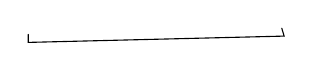
\begin{tikzpicture}[x=1cm,y=1cm,baseline=(current bounding box.center),line cap=round]\draw (0,.1)--(0,0)--(3.25,.08)--(3.22,.18);\end{tikzpicture}}{\frac{f'(re^{i\varphi})}{f(re^{i\varphi})}e^{i\varphi}\,dr}}\ (r\mu(r))
\end{aligned}
\]
\[
\int_a^b=\left[r\mu(r)\log f(re^{i\varphi})\right]_a^b-\int_a^b\log f(re^{i\varphi})\,d(r\mu(r))
\]
(en supposant $\mu(r)$ continûment différentiable)

-- On choisit brutalement la détermination
principale du logarithme -- pas de trou-\newline
ble, car les intégrales \deleted{\unsure{si elles ont|simplement}} doubles
qui interviennent sont convergentes)
\figure{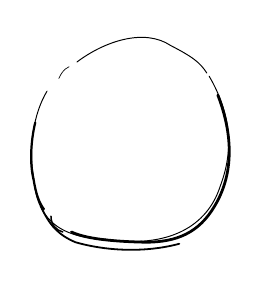
\begin{tikzpicture}[x=.01cm,y=-.01cm,line cap=round,line join=round]
\draw[line width=.35pt] (77,51) .. controls (113,24) and (163,8) .. (196,30) .. controls (223,44) and (233,51) .. (242,65);
\draw[line width=.25pt] (67,57) .. controls (60,60) and (56,67) .. (54,72);
\draw[line width=.35pt] (39,88) .. controls (22,116) and (15,160) .. (22,197) .. controls (25,248) and (52,274) .. (112,276) .. controls (194,289) and (243,259) .. (259,209) .. controls (278,159) and (271,114) .. (245,69);
\draw[line width=.8pt] (24,128) .. controls (18,153) and (17,181) .. (22,201) .. controls (25,219) and (29,230) .. (35,238);
\draw[line width=1pt] (256,93) .. controls (276,145) and (276,194) .. (252,234) .. controls (232,268) and (204,280) .. (164,280) .. controls (118,279) and (87,275) .. (70,267);
\draw[line width=.65pt] (31,234) .. controls (42,259) and (54,271) .. (75,280) .. controls (117,292) and (166,293) .. (207,282);
\draw[line width=.55pt] (44,247) .. controls (44,258) and (51,265) .. (59,267);
\end{tikzpicture}}
D'où, en substituant, intervertissant les signes $\int\!\int$, et
\margin{en prenant les parties réelles}
\[
\hbox{\begingroup\setbox0=\hbox{$\displaystyle \displaystyle \deleted{2\pi}\int_{\unsure{a}}^b n(r)\mu(r)\,dr\unsure{:|=}\left[r\mu(r)V(r)\right]_a^b-\int_a^b V(r)\,d(r\mu(r))$}\kern5pt\rlap{\tikz[baseline=0pt]{\draw[line width=.35pt] (-4pt,\the\dimexpr\ht0+4pt\relax)--(\the\dimexpr\wd0+5pt\relax,\the\dimexpr\ht0+4pt\relax);\draw[line width=.4pt] (-5pt,\the\dimexpr\ht0+1pt\relax)--(-4pt,\the\dimexpr-\dp0-1pt\relax);\draw[line width=.4pt] (-4pt,\the\dimexpr-\dp0-3pt\relax)--(-4pt,\the\dimexpr-\dp0-4pt\relax)--(-1pt,\the\dimexpr-\dp0-4pt\relax);\draw[line width=.35pt] (1pt,\the\dimexpr-\dp0-4pt\relax)--(\the\dimexpr\wd0+2pt\relax,\the\dimexpr-\dp0-4pt\relax);\draw[line width=.35pt] (\the\dimexpr\wd0+5pt\relax,\the\dimexpr\ht0+1pt\relax)--(\the\dimexpr\wd0+5pt\relax,\the\dimexpr-\dp0-1pt\relax);}}\copy0\kern6pt\endgroup}
\]
où \qquad \uline{$\displaystyle V(r)=\frac1{2\pi}\int_0^{2\pi}\log|f(re^{i\varphi}\unsure{\vert|)}\,d\varphi$}
Prenons $\mu(r)=-\lambda'(r)$, on obtient \enspace $(0<a<b<+\infty$
\[
\hbox{\begingroup\setbox0=\hbox{$\displaystyle \begin{aligned}
\sum_{\substack{\nu\unsure{,}\\a<r_\nu<b}}\lambda(r_\nu)^{\deleted{\unsure{\alpha}}}
&=\lambda^{\unsure{\mathord{-}|'}}(b)n(b-0)-\lambda(a)n(a+0)+[r\mu(r)V(r)]_a^b\deleted{\unsure{+\int^b V(r)\,d(r\mu|+\int^b}}\\
&\qquad+\int_a^b V(r)\,d(r\lambda'(r))
\end{aligned}$}\kern5pt\rlap{\tikz[baseline=0pt]{\draw[line width=.35pt] (-4pt,\the\dimexpr\ht0+4pt\relax)--(\the\dimexpr\wd0+5pt\relax,\the\dimexpr\ht0+4pt\relax);\draw[line width=.4pt] (-5pt,\the\dimexpr\ht0+1pt\relax)--(-4pt,\the\dimexpr-\dp0-1pt\relax);\draw[line width=.35pt] (-1pt,\the\dimexpr-\dp0-4pt\relax)--(\the\dimexpr\wd0+2pt\relax,\the\dimexpr-\dp0-4pt\relax);\draw[line width=.4pt] (\the\dimexpr\wd0+5pt\relax,\the\dimexpr-\dp0+5pt\relax)--(\the\dimexpr\wd0+5pt\relax,\the\dimexpr-\dp0-4pt\relax);}}\copy0\kern6pt\endgroup}
\]
\margin{119}


\scanpage{119}
(Si $r^2\mu(r)\to0$ pour $r\to0$, et $|f(0)|=1$, on a
\[
\sum_{r_\nu<b}\lambda(r_\nu)=\lambda(b)n(b-0)\deleted{\unsure{+}}-b\lambda'(b)V(b)+\int_0^b V(r)\,d(r\lambda'(r))\quad\big)
\]

Comme $|V(r)|\leq M(r)=\mathop{\rm Sup}_{|z|:r}|f(z)|$, on obtient une
majoration de $\deleted{\sum\lambda}\unsure{\deleted{(r_\nu)}|(r_\nu)}$ $\int_a^b n(r)\mu(r)\,dr$ en fonction
de $M(r)$
\margin{120}


\scanpage{120}
\uline{Sur une certaine fonction holomorphe \deleted{\unsure{de variable|définie}} \inserted{sur l'}espace de Banach $l^1$.}

Soit, pour $\lambda=(\lambda_i)\in l^1$ et tout entier $n>0$
\[
\alpha_n(\lambda)=\sum_{i_1<\mathord{-}\mathord{.}\mathord{.}<i_n}\lambda_{i_1}\mathord{.}\mathord{-}\lambda_{i_n}
\]
On a
\[
\alpha_n(\lambda)\leq\frac{\|\lambda\|_1^n}{n!}
\]
les $\alpha_n(\lambda)$ sont les coefficients de la fonction entière
de genre zéro
\[
f(\unsure{n|\lambda})=\prod_1(1+\lambda_i z)
\]
et on obtient, à un facteur \unsure{constant} près, les
coefficients les plus généraux d'une fonction entière
de genre zéro.

\uline{Proposition} Pour tout $\lambda\in l^1$, la série $\sum_0^\infty n!\alpha_n(\lambda)$
\margin{\tikz[x=1pt,y=1pt]{\draw[line width=.45pt] (0,0)--(.6,-32)--(2,-67)--(3.2,-101);}}
est absolument convergente, soit $S(\lambda)$ sa somme.
La fonction $\lambda\to S(\lambda)$ est holomorphe au voisinage
de $0$, avec un rayon de convergence égal à $1$,
\deleted{\unsure{ce qui fait que ses|ce qui fait que sur}} \inserted{et ses restrictions} aux sous-espaces vectoriels
complexes de dim finie sont holomorphes.
Cependant, \deleted{elle} cette fonction n'est pas bornée
dans la boule unité de $l^1$, et n'est par
suite pas une fonction entière de $\lambda$.

\uline{Corollaire} On a \inserted{pour $\lambda\in l^1$} $\sqrt[n]{n!|\alpha_n(\lambda)|}\to 0$,
\margin{\tikz[x=1pt,y=1pt]{\draw[line width=.45pt] (0,0)--(-.5,-14)--(.4,-38)--(1.5,-69);}}
$\sqrt[n]{|\alpha_n(\lambda)|}=o\left(\frac{1}{n}\right)$, $\alpha_n(\lambda)=\frac{\varepsilon_n^n}{n!}$ avec $\varepsilon_n\to 0$
Si $\sum a_nz^n$ est une fonction entière de
genre zéro, la suite des $a_n$ jouit
des $=\mathrm s$ propriétés

En effet, $\sqrt[n]{n!|\alpha_n(\lambda)|}\to 0$ exprime que
\margin{121}


\scanpage{121}
\[ \sum n!\alpha_n(\lambda z)=\sum n!\alpha_n(\lambda)z^n \]
converge
quel que soit $z$. Les deux \inserted{autres} relations
\deleted{\unsure{sont|mais}} sont une autre façon d'exprimer la première,
-- en tenant compte de la formule de
Stirling $\sqrt[n]{n!}\sim\frac{n}{e}$ --.

Démonstration de la proposition. On peut
supposer les $\lambda_i>0$ \inserted{et \uline{décroissants}} $]$ soit alors $f(z)=\prod(1+\lambda_i z)$
\deleted{\unsure{une fonction}}, \inserted{$=\sum\alpha_n\deleted{(\lambda)}z^n$} \inserted{(où on pose $\alpha_n=\alpha_n(\lambda)$)} on a, \deleted{\unsure{en vertu de}} l'inégalité
de Cauchy
\[ \alpha_n\leq\frac{M(R)}{R^{n+1}}\qquad\text{pour tout }R>0 \]
où $M(R)$ est le maximum de $|f(z)|$ sur la
circonférence $|z|=R$, \unsure{d'où|d'ici|donc} $M(R)=\prod(1+\lambda_iR)$.
\deleted{Soit} On a donc
\[ \alpha_n\leq\left(\frac1R+\lambda_1\right)\mathord{-}\left(\frac1R+\lambda_{n+1}\right)\prod_{i=n+2}^{\infty}(1+\lambda_i R) \]
\deleted{\unsure{un facteur}} \inserted{Or} $\prod_{i=n+2}^{\infty}(1+\lambda_i R)\leq e^{\rho_{n+1}R}$, où
$\rho_{n+1}=\sum_{k=n+2}^{\infty}\lambda_k$. faisons $R=\frac{n+1}{\rho_{n+1}}$, on obtient
\[ \begin{aligned}
\alpha_n&\leq\left(\frac{\rho_{n+1}}{n+1}+\lambda_1\right)\mathord{-}\,\mathord{-}\left(\frac{\rho_{n+1}}{n+1}+\lambda_{n+1}\right)e^n \deleted{\unsure{\leq(\frac{\rho_1}{1}+\lambda_1)\mathord{-}\,\mathord{-}(\frac{\rho_{n+1}}{}}}\\
&\leq\left(\frac{\unsure{\rho_2|\rho_1}}{1}+\lambda_1\right)\left(\frac{\rho_2}{2}+\lambda_2\right)\mathord{-}\,\mathord{-}\left(\frac{\rho_{n+1}}{n+1}+\lambda_{n+1}\right)e^n
\end{aligned} \]
Or, \deleted{\unsure{comme les}} \inserted{les} $\lambda_i$ \deleted{\unsure{sont}} \unsure{étant|formant} décroissants et leur
suite sommable, on a $\lambda_n=o(\frac1n)$, d'autre part on
a \deleted{$\unsure{\rho_n\leq 0|\rho_n\to 0}$} $\frac{\rho_n}{n}=\uline{o}(\frac{1}{n})$, d'où $\frac{\rho_n}{n}+\lambda_n\leq\frac{\varepsilon_{n+1}}{n}$, où $\varepsilon_n\to0$
\[ \alpha_n\leq\frac{\varepsilon_0\varepsilon_{\unsure{2|0|1}}\mathord{-}\varepsilon_{n+1}}{(n+1)!}e^n\qquad\text{où }\varepsilon_i\to0. \]
D'où
\margin{122}


\cotefile{1}
\scanpage{122}
\[
n!\alpha_n\leq\frac{\varepsilon_0}{n+1}\,
\varepsilon_1\mathord{-}\mathord{-}\varepsilon_n\,e^n
\qquad
\sqrt[n]{n!\alpha_n}\leq e\left(\frac{\varepsilon_0}{n+1}\right)^{1/n}
\deleted{\unsure{\varepsilon_1\ldots\varepsilon_n}}
\inserted{(\varepsilon_1\mathord{-}\varepsilon_n\unsure{,}}
\]
$\unsure{(}n\to\infty$,
$\left(\frac{\varepsilon_0}{n+1}\right)^{1/n}\to1$, et
$(\varepsilon_1\mathord{.}\mathord{.}\varepsilon_n)^{1/n}\to0$,
comme on voit immédiatement, d'où $\sqrt[n]{n!\alpha_n}\to0$,
d'où suit que $\sum n!\alpha_n(\lambda)$ converge absolument
\unsure{$\lambda$|à}. Il en résulte
\margin{\unsure{pour tout sous-espace|sur tout sous-espace} de dimension finie $\unsure{F|E}\unsure{\subset|\text{de}}l^1$,
la fonction $S(\lambda)$ est holomorphe
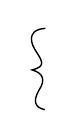
\begin{tikzpicture}[x=.008cm,y=.008cm]
\draw[line width=.5pt] (30,129) .. controls (7,128) and (3,113) .. (13,96)
.. controls (25,77) and (32,69) .. (9,63)
.. controls (26,58) and (31,48) .. (20,31)
.. controls (10,14) and (13,3) .. (29,0);
\end{tikzpicture}}

Comme on a $|\alpha_n(\lambda)|\leq\|\lambda\|_1^n$, il suit que
la fonction $S(\lambda)$ \inserted{sur $l^1$}
\begin{tikzpicture}[x=.012cm,y=.012cm,baseline=-.3ex]
\draw[line width=.45pt] (64,65) .. controls (77,54) and (61,41) .. (34,36)
.. controls (13,34) and (8,25) .. (4,0);
\end{tikzpicture}
est holomorphe au voisinage
de l'origine\,; d'ailleurs, la forme $n$ fois linéaire
$\alpha_n(\lambda^{(1)},\mathord{-},\lambda^{(n)})$ associée à
$\lambda\to\alpha_n(\lambda)$ est
\[
\alpha_n(\lambda^{(1)}\unsure{\mathord{.}\mathord{.}|\ldots}\lambda^{(n)})
=\frac{1}{n!}\sum_{i_1,\mathord{-},i_n}
\lambda^{(1)}_{i_1}\mathord{.}\mathord{-}\lambda^{(n)}_{i_n}
\]
(la somme étant étendue aux systèmes $(i_1\mathord{-}i_n)$ d'indices distincts)
d'où $\|\alpha_n\|\leq\frac{1}{n!}$
\inserted{soit $\unsure{\|}\deleted{\unsure{\alpha_n}}n!\alpha_n\|\leq1$}
\begin{tikzpicture}[x=.018cm,y=.018cm,baseline=-.5ex]
\draw[line width=.45pt] (0,0) .. controls (4,12) and (10,18) .. (16,19)
-- (85,19) .. controls (100,19) and (105,24) .. (106,27);
\end{tikzpicture},
le rayon de convergence
strict \inserted{$R_0$} de la fonction $S(\lambda)$ à l'origine est
donc \deleted{\unsure{$R_0$|être|à peu}} $\geq1$.
Soit \inserted{alors} $a_{\deleted{\unsure{m}}}^{(m)}$ l'élément de $l^1$
\deleted{\unsure{égal à}} donné par
\[
a_i^{(m)}=\begin{cases}
\frac{1}{m}&\text{si }i\leq m\\
0&\text{si }i>m
\end{cases}
\]
on a manifestement $\|a^{(m)}\|_1=1$, et
\[
\alpha_n(a^m)=\deleted{\unsure{\frac{1}{m^n}}}
\left\{\begin{aligned}
&\deleted{\unsure{0\quad\text{si }n>m}}\\
&\frac{1}{m^n}\frac{m!}{n!(m-n)!}\quad\text{si }n\leq m
\end{aligned}\right.\,,\quad\text{d'où}
\]
\[
n!\alpha_n(a^m)=\frac{1}{m^n}\,m(m-1)\mathord{-}(m-n+1)
=\unsure{\deleted{1}|\lbrace}
(1-\tfrac{1}{m})(1-\tfrac{\unsure{3|2}}{m})
\mathord{.}\mathord{-}(1-\tfrac{n-1}{m})
\]
Donc $n!\alpha_n(a^{(m)})\to1$ pour $m\to\infty$.
Il suit que $S(a^{(m)})\to\infty$ si $m\to\infty$ ;
donc $S(\lambda)$ n'est pas borné dans la boule
unité de $l^1$, et son rayon de convergence
large \inserted{$R_1$} à l'origine est donc aussi $\leq1$, d'où $R_0=R_1=1$.

\deleted{Enfin, $S(\lambda)$ étant holomorphe au voisinage de
\unsure{$0$|$a$} et pouvant être \unsure{holomorphe|prolongée|holomorphes}
sur \unsure{chaque droite}}
\margin{123}


\scanpage{124}
\[
\bigl(\|u_1\wedge\cdots\wedge u_n\|_1\bigr)^2\leq
\unsure{\surd}\alpha_n(|u_1|\wedge\mathord{-}\mathord{-}\mathord{-}\mathord{-}\wedge|u_n|)
\,\alpha_n(|u_1^+|',\cdot\mathord{-}\mathord{-}
\deleted{\unsure{\sqrt{\vphantom{u}}}}|u_n^{\deleted{\unsure{+}}}|^{\unsure{'}})
\]
\[
|\alpha_n u_1\unsure{\wedge|,}\cdot\mathord{-}u_n)|
\leq\alpha_n(|u_1|,\cdot\cdot\mathord{-}|u_n|).
\]
\begin{flushright}
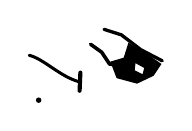
\begin{tikzpicture}[x=1cm,y=1cm,line cap=round,line join=round]
\draw[line width=1.1pt] (0,.2) .. controls (.18,.16) and (.4,-.08) .. (.65,-.14);
\draw[line width=1.5pt] (.65,-.02)--(.64,-.25);
\fill (.12,-.37) circle (.035);
\draw[line width=1.2pt] (.95,.53)--(1.17,.46)--(1.42,.27)--(1.69,.13);
\draw[line width=1.3pt] (.78,.34)--(.92,.24)--(1.02,.09)--(1.22,.06);
\fill[even odd rule] (1.03,.12)--(1.2,.17)--(1.26,.36)--(1.48,.23)--(1.68,.09)--(1.58,-.06)--(1.37,-.16)--(1.11,-.09)--cycle
 (1.35,.1)--(1.46,.04)--(1.44,-.04)--(1.34,.01)--cycle;
\end{tikzpicture}
\end{flushright}

\uline{Démonstration} \quad Posons $u_i=\sum_\alpha\lambda_\alpha^{(i)}a_\alpha^{(i)}\otimes b_\alpha^{(i)}$
(représentation canonique de $u_i$) alors
\margin{$\unsure{\mathrm I}$}
\[
|u_i|=\sum_\alpha\lambda_\alpha^{(i)}a_\alpha^{(i)},\qquad
|u_i|'=\sum_\alpha\lambda_\alpha^{(i)}b_\alpha^{(i)}
\]
\[
u_1\wedge\cdot\mathord{-}\mathord{-}\wedge u_n
=\frac{1}{n!}\sum_{\alpha_1\mathord{-}\alpha_n}
\lambda_{\alpha_1}^{(1)}\cdot\mathord{-}\lambda_{\alpha_n}^{(n)}
(a_{\alpha_1}^{(1)}\wedge\cdot\cdot\wedge a_{\alpha_n}^{(n)})
\otimes(b_{\alpha_1}^{(1)}\wedge\cdots\wedge b_{\alpha_{\unsure{n}}}^{\unsure{(n}}
\]
d'où
\[
\|u_1\wedge\cdot\mathord{-}u_n\|_1\leq\frac{1}{n!}\sum_{\alpha_1\mathord{-}\alpha_n}
\lambda_{\alpha_1}^{(1)}\mathord{-}\lambda_{\alpha_n}^{(n)}
\|a_{\alpha_1}^{(1)}\wedge\mathord{-}\wedge a_{\alpha_n}^{(n)}\|
\|b_{\alpha_1}^{(1)}\wedge\mathord{-}\wedge b_{\alpha_n}^{(n)}\|
\]
d'autre part on a, par le $=$ calcul
\[
\begin{aligned}
\alpha_n(|u_1|,\mathord{-}|u_n|)&\inserted{=\operatorname{Tr}|u_1|\wedge\mathord{-}|u_n|}=
\frac{1}{n!}\sum_{\alpha_1\mathord{-}\alpha_n}\lambda_{\alpha_1}^{(1)}\mathord{-}\lambda_{\alpha_n}^{(n)}
\|a_{\alpha_1}^{(1)}\wedge\mathord{-}a_{\alpha_n}^{(n)}\|^2
\deleted{\unsure{b_{\alpha_1}^{(1)}\wedge\ldots\wedge a_{\alpha_n}^{(n)}}}\\
\alpha_n(|u_1|',\cdot\mathord{-}|u_n|')&=\frac{1}{n!}\sum_{\alpha_1\mathord{-}\alpha_n}
\lambda_{\alpha_1}^{(1)}\mathord{-}\lambda_{\alpha_n}^{(n)}
\|b_{\alpha_1}^{1}\wedge\mathord{-}\wedge b_{\alpha_n}^{(n)}\|^2
\end{aligned}
\]
\margin{$\unsure{\lambda|\alpha}_n=$}
L'inégalité voulue \deleted{\unsure{est}} \unsure{:|est} alors conséquence de l'inégalité
\[
\deleted{\unsure{(a_{\alpha_1}^{(1)}\wedge\ldots\wedge a_{\alpha_n}^{(n)},b_{\alpha_1}^{(1)}\wedge\ldots\wedge b_{\alpha_n}^{(n)})}}
\]
\margin{$\unsure{\mathrm{II}}$}
de Cauchy-Schwartz.

\par\medskip\noindent
\hbox{\rlap{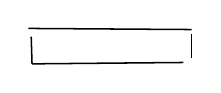
\begin{tikzpicture}[baseline=0pt,x=1em,y=1em,line width=.55pt]
\draw (-.1,1)--(5.8,.96);
\draw (0,.7)--(.03,-.28);
\draw (.03,-.28)--(5.5,-.23);
\draw (5.8,.81)--(5.8,-.06);
\end{tikzpicture}}\kern.25em Corollaire 1\kern.45em}
\[
|\alpha_n\unsure{(}u_1,\mathord{-}u_n)|\leq\|u_1\wedge\mathord{-}\wedge u_n\|_1
\leq\frac{1}{2}\bigl(\alpha_n(|u_1|,\cdot\mathord{-}|u_n|)+\alpha_n(|u_1|',\mathord{-}\mathord{-}|u_n|')\bigr)
\]

\par\medskip\noindent
\hbox{\rlap{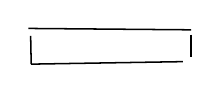
\begin{tikzpicture}[baseline=0pt,x=1em,y=1em,line width=.55pt]
\draw (-.08,1)--(5.8,.95);
\draw (0,.73)--(.02,-.29);
\draw (.02,-.29)--(5.5,-.2);
\draw (5.8,.78)--(5.8,-.04);
\end{tikzpicture}}\kern.25em Corollaire 2\kern.45em}
\[
|\alpha_n(A+B)|^2\leq\deleted{\unsure{\sqrt{\vphantom A}}}\alpha_n(|A|+|B|)
\alpha_n(|A^{\unsure{*}}|'+|B^{\unsure{*}}|^{\unsure{+|'}})
\]
En effet, on a \deleted{\unsure{$\alpha_n(A+B$}}
\[
\begin{aligned}
|\alpha_n(A+B)|^{\unsure{2}}&=\left|\sum_k C_k^n\alpha_n(\overbrace{A,\mathord{-}A}^{k},
\overbrace{B,\mathord{-}B}^{n-k})\right|^{\unsure{2}}\\
&\leq\deleted{\unsure{\surd}}\sum_k C_k^n
\bigl(\alpha_n(\overbrace{|A|,\mathord{-}\unsure{A|\lvert A}}^{k},\overbrace{\unsure{\lvert A\rvert|\lvert B\rvert},\mathord{-}\unsure{B_1|B,|\lvert B\rvert}}^{n-k})\bigr)^{1/2}
\bigl(\sum_k\alpha_n(\overbrace{|A|',\mathord{-}|A|'}^{k},|B|'\mathord{-}\mathord{-})\bigr)^{1/2}
\end{aligned}
\]
\margin{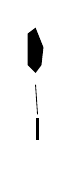
\begin{tikzpicture}[x=.025cm,y=-.025cm]
\fill (0,0)--(4,-3)--(8,7)--(7,16)--(4,20)--(0,16)--cycle;
\draw[line width=.3pt] (4,26)--(5,41);
\draw[line width=.8pt] (5,43)--(5,54);
\end{tikzpicture}}
d'où, par l'inégalité de Cauchy-Schwartz
\[
|\alpha_n(A+B)|^{\unsure{2}}\leq\bigl(\sum_k C_k^n\alpha_n
\unsure{\lvert A\rvert,\mathord{-}\lvert A\rvert,\lvert B\rvert\mathord{-}B,)|
(\lvert A\rvert,\mathord{-}\lvert A\rvert,\lvert B\rvert\mathord{-}B,)}\bigr)^{1/2}
\bigl(\sum_k{}'\quad\bigr)^{\unsure{1/2}}\unsure{!}
\]
\margin{125}
